\documentclass[tikz,border=2pt]{standalone}
\usepackage{amsmath}
\usetikzlibrary{arrows.meta}
\begin{document}
% Element-wise comparison: x = 1..6 compared with 4 gives F F F F T T;
% z = (2, NA, 7) compared with 5 gives F NA T (a comparison with NA is NA).
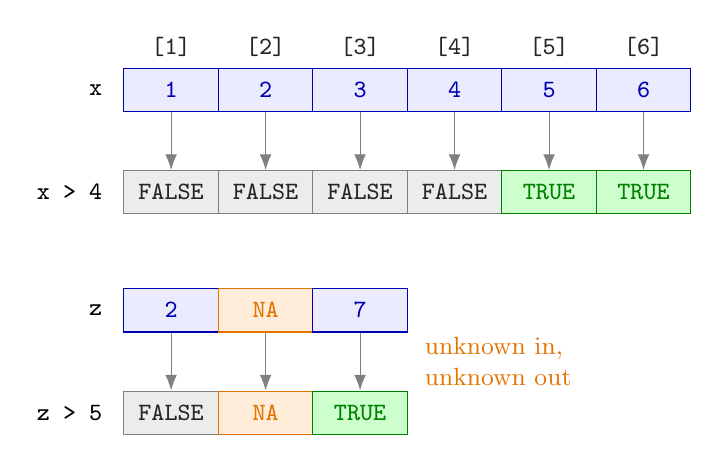
\begin{tikzpicture}[font=\small, >={Latex[length=2mm]},
  cell/.style={draw, minimum width=1.2cm, minimum height=0.55cm, inner sep=1pt, font=\small\ttfamily},
  val/.style={cell, draw=blue!70!black, fill=blue!8, text=blue!70!black},
  yes/.style={cell, draw=green!50!black, fill=green!20, text=green!50!black},
  no/.style={cell, draw=gray, fill=gray!15, text=gray!30!black},
  na/.style={cell, draw=orange!90!black, fill=orange!15, text=orange!90!black},
  lab/.style={anchor=east, font=\small\ttfamily},
  idx/.style={gray!30!black, font=\small\ttfamily}]
  % upper panel: x > 4
  \node[lab] at (0.45,0) {x};
  \foreach \v [count=\i] in {1,2,3,4,5,6} {
    \node[val] (a\i) at (1.2*\i,0) {\v};
    \node[idx] at (1.2*\i,0.55) {[\i]};
  }
  \node[lab] at (0.45,-1.3) {x > 4};
  \foreach \s/\t [count=\i] in {no/FALSE,no/FALSE,no/FALSE,no/FALSE,yes/TRUE,yes/TRUE} {
    \node[\s] (b\i) at (1.2*\i,-1.3) {\t};
    \draw[->, gray] (a\i.south) -- (b\i.north);
  }
  % lower panel: z > 5 with a missing value
  \node[lab] at (0.45,-2.8) {z};
  \foreach \s/\t [count=\i] in {val/2,na/NA,val/7} {
    \node[\s] (c\i) at (1.2*\i,-2.8) {\t};
  }
  \node[lab] at (0.45,-4.1) {z > 5};
  \foreach \s/\t [count=\i] in {no/FALSE,na/NA,yes/TRUE} {
    \node[\s] (d\i) at (1.2*\i,-4.1) {\t};
    \draw[->, gray] (c\i.south) -- (d\i.north);
  }
  \node[anchor=west, orange!90!black, align=left] at (4.3,-3.45) {unknown in,\\ unknown out};
\end{tikzpicture}
\end{document}
